% ==============================================================================
% Section 4.6: CED Alignment
% ==============================================================================
\subsection{CED Alignment}
\label{sec:ced}

In March 2026, the UN Committee on Enforced Disappearances (CED) issued its first-ever referral to the General Assembly under Article~34 of the Convention, finding that enforced disappearances in Mexico constitute crimes against humanity \citep{CED_MEX_art34_2026}.
The decision identifies ``multiple attacks at different moments and in different parts of the territory'' and names eight states as particular loci of concern.
Our LISA analysis provides the first national-scale quantitative evidence bearing on these geographic claims.

Figure~\ref{fig:ced_states} presents the HH dynamics for the eight CED-named states.

\begin{figure}[htbp]
  \centering
  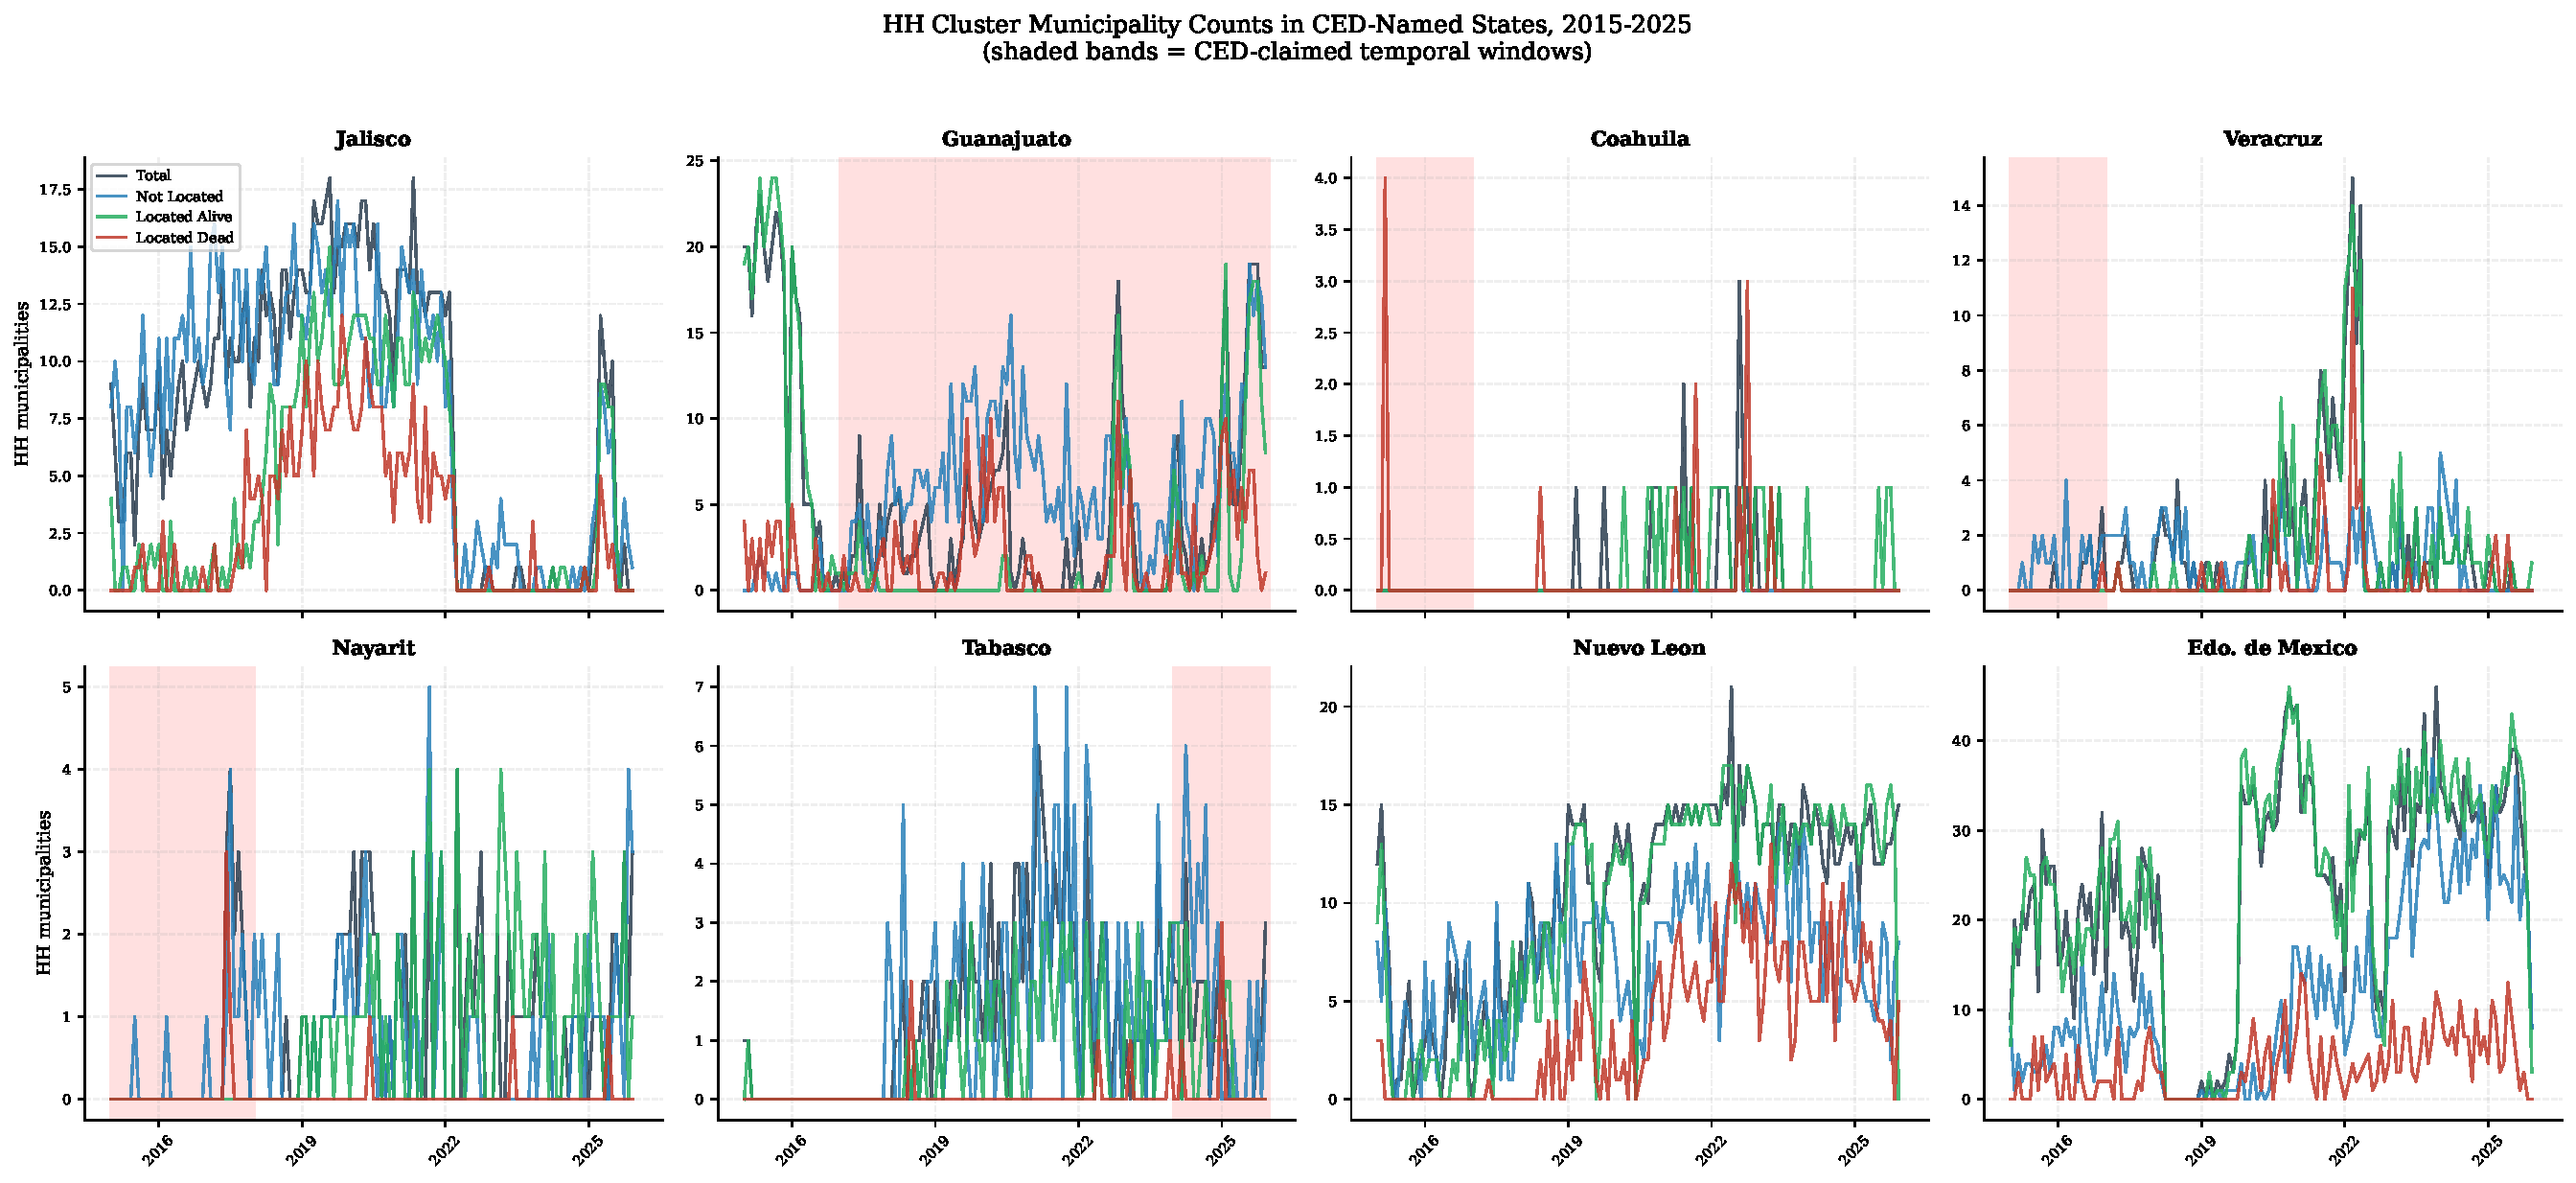
\includegraphics[width=\textwidth]{figures/fig9_ced_states.pdf}
  \caption{Monthly count of HH municipalities in eight CED-named states by outcome status, \studyperiod{}.
           Shaded bands indicate CED-referenced temporal windows.}
  \label{fig:ced_states}
\end{figure}

\textbf{Estado de M\'{e}xico} shows the strongest growth of any CED-named state: Not Located HH municipalities increased at $+2.36$ per year ($p < 0.001$), and Located Alive at $+1.81$ per year ($p < 0.001$).
The CED's temporal window (2015--2025) is fully aligned with the observed expansion.

\textbf{Nuevo Le\'{o}n} exhibits robust multi-status growth: Located Alive $+1.34$/yr ($p < 0.001$) and Located Dead $+0.80$/yr ($p < 0.001$).
HH peaks occur in 2022--2023, consistent with civil society reports of intensified organized criminal activity in the Monterrey metropolitan area.

\textbf{Guanajuato} presents a compositional shift.
Not Located HH municipalities are rising ($+0.75$/yr, $p < 0.001$), but Located Alive is declining ($-0.57$/yr, $p < 0.001$).
The CED's characterization of an ``eightfold increase since 2017'' aligns with the Not Located trajectory but not with the Located Alive decline---fewer people are being found alive even as more remain not located.

\textbf{Jalisco} shows declining HH municipalities across all statuses, with peaks around 2019.
This appears to contradict the CED's characterization of Jalisco as ``currently highest'' in disappearances; however, our HH metric captures spatial \emph{clustering}, not absolute volume.
A state may have high absolute counts but spatially diffuse registrations that do not produce significant local clusters.

\textbf{Coahuila, Veracruz, and Nayarit} show low or zero HH municipalities throughout most of the study period.
The CED's temporal claims for these states reference crisis periods (2009--2017) that largely predate or fall at the beginning of our study window, limiting our ability to capture the dynamics the CED describes.

\textbf{Tabasco} is flagged by the CED for an ``exponential increase 2024--2025'' with specific concern for girls and women.
Our sex-disaggregated analysis provides partial support: female Located Alive HH municipality-months (31) substantially exceed male (6) in 2023--2025, consistent with the CED's claim of gendered victimization.
For Not Located, however, the pattern is reversed (male 39 municipality-months vs.\ female 34), and overall HH counts in Tabasco remain low.

We emphasize three caveats.
First, we do not adjudicate state responsibility; our analysis is descriptive.
Second, the RNPDNO aggregates all disappearances, not only enforced disappearances---the government's position is that many registered cases reflect non-state-actor crimes.
Our spatial clusters capture the composite phenomenon regardless of perpetrator type.
Third, several CED-named states exhibit low HH counts not because disappearances are absent but because the RNPDNO may undercount registrations in states with weaker institutional infrastructure.
